\documentclass[10pt,twocolumn,letterpaper]{article}
\usepackage[T1]{fontenc}
\usepackage{mathptmx}
\usepackage[scaled=1]{helvet}
\usepackage[left=17.3mm,right=17.3mm,top=16.5mm,bottom=14mm,
  columnsep=4.2mm,headheight=10pt,headsep=9pt]{geometry}
\usepackage{amsmath,graphicx,booktabs,tabularx}
\usepackage{caption,microtype,fancyhdr,placeins,titlesec,xcolor,dblfloatfix}
\definecolor{PaperInk}{RGB}{0,0,0}
\definecolor{LinkBlue}{RGB}{0,64,135}
\usepackage[colorlinks=true,linkcolor=LinkBlue,citecolor=LinkBlue,
  urlcolor=LinkBlue]{hyperref}
\urlstyle{same}

\hypersetup{pdftitle={Satellite Flood Mapping and Road Access in Mountain Valleys}}
\newcolumntype{L}{>{\raggedright\arraybackslash}X}
\newcolumntype{P}[1]{>{\raggedright\arraybackslash}p{#1}}
\newcommand{\km}{\,\mathrm{km}}
\newcommand{\m}{\,\mathrm{m}}
\newcommand{\dash}{\textemdash}
\setlength{\parindent}{1em}
\setlength{\parskip}{0pt}
\setlength{\tabcolsep}{3.5pt}
\renewcommand{\arraystretch}{1.1}
\captionsetup{font={sf,footnotesize},labelfont={color=PaperInk},skip=5pt}
\renewcommand{\thesection}{\Roman{section}}
\renewcommand{\thesubsection}{\thesection.\Alph{subsection}}
\titleformat{\section}{\centering\sffamily\bfseries\fontsize{10.5}{12}\selectfont\color{PaperInk}}
  {\thesection.}{0.6em}{\MakeUppercase}
\titleformat{\subsection}{\sffamily\bfseries\itshape\fontsize{10}{12}\selectfont\color{PaperInk}}
  {\Alph{subsection}.}{0.5em}{}
\titlespacing*{\section}{0pt}{13pt plus 2pt minus 2pt}{7pt}
\titlespacing*{\subsection}{0pt}{10pt plus 2pt minus 1pt}{6pt}
\setlength{\textfloatsep}{11pt plus 2pt minus 2pt}
\setlength{\floatsep}{10pt plus 2pt minus 2pt}
\setlength{\intextsep}{10pt plus 2pt minus 2pt}
\renewcommand{\topfraction}{0.9}
\renewcommand{\bottomfraction}{0.85}
\renewcommand{\textfraction}{0.08}
\renewcommand{\floatpagefraction}{0.75}
\renewcommand{\dbltopfraction}{0.95}
\renewcommand{\dblfloatpagefraction}{0.65}
\setcounter{topnumber}{5}
\setcounter{dbltopnumber}{5}
\setcounter{totalnumber}{10}
\raggedbottom
\pagestyle{fancy}
\fancyhf{}
\fancyhead[L]{\sffamily\fontsize{7}{8}\selectfont Satellite flood mapping and road access}
\fancyhead[R]{\sffamily\fontsize{7}{8}\selectfont\thepage}
\renewcommand{\headrule}{\hbox to\headwidth{\color{PaperInk}\leaders\hrule height 0.4pt\hfill}}
\emergencystretch=1em
\clubpenalty=10000
\widowpenalty=10000
\renewenvironment{abstract}{\par\noindent\begingroup\sffamily\bfseries
  \fontsize{9}{10.5}\selectfont\textcolor{PaperInk}{\itshape Abstract---}}
  {\par\endgroup\vspace{8pt}}

\title{\normalfont\sffamily\fontsize{24}{28}\selectfont\color{PaperInk}
  Satellite Flood Mapping and Road Access\\in Mountain Valleys}
\author{\sffamily Sadat Bashir and Adfar Jaan\\[3pt]\sffamily\small riwaq}
\date{}

\begin{document}
\maketitle
\thispagestyle{fancy}
\begin{abstract}
Mountain floods leave water and deposited debris along the valley floor, while cloud and radar
shadow prevent parts of the valley from being observed. Sentinel-1 backscatter change, Sentinel-2
spectral change and water segmentation are combined on a 10 m grid, with slope and height above
drainage restricting detections on the valley sides. The flood extent is compared with pre-event
OpenStreetMap buildings, roads and bridges, and affected road segments are removed before settlement
road access is calculated. For the Bhote Koshi--Trishuli flood of 26 August 2026, the extent has F1
0.906 against four Copernicus EMSR927 areas, and the road-access calculation identifies 10,788
buildings without a road connection. Trishuli was used to select settings during development. The
27-event evaluation gives mean F1 0.546, whereas the three test events excluded from parameter
selection have mean F1 0.366. Excluding snow from optical date selection changes the
twelve-event development mean from 0.5335 to 0.5351; two additional flood cases have unchanged
results.
\end{abstract}

{\noindent\sffamily\bfseries\fontsize{9}{10.5}\selectfont
\textcolor{PaperInk}{\itshape Index Terms---}Flood extent, Sentinel-1, Sentinel-2, debris,
road access, mountain valleys.\par}

\section{Introduction}
Flood water can recede before a clear satellite image is acquired, leaving debris on the valley
floor that is absent from an open-water segmentation. The debris can increase radar backscatter,
whereas smooth water often decreases it, so a decrease in backscatter alone does not describe the
affected ground. Cloud removes optical observations and steep valley sides also cause radar shadow
and layover. These conditions require the measured changes to be considered with the terrain and
with the ground that remains unobserved.

We compare satellite images acquired before and after the event and combine the change detections
with radar and optical water predictions. Height above drainage and channel connections limit
detections on the slopes; on large low plains, where water may already be present before the event,
the water predictions are used without requiring additional change. Buildings, roads and bridges are
taken from pre-event OpenStreetMap. Removing affected segments from the road network then allows a
settlement outside the mapped flood extent to be identified when its road connection has been lost.
The Bhote Koshi--Trishuli flood is used as the case study, with further comparisons on mountain and
lowland events.

\section{Data and image processing}
\subsection{Input data}
Sentinel-1 GRD is calibrated and terrain corrected from the ESA annotations (Table~\ref{tab:data}).
The OpenStreetMap snapshot must precede the event, including the wider network used for road access;
its replication time is checked before buildings and roads are read. Copernicus EMS and UNOSAT
geometries are excluded from the mapping inputs and read separately for evaluation.

\begin{table}[!htb]
\caption{Input data and processing.}
\label{tab:data}
\fontsize{8.2}{9.6}\selectfont
\begin{tabularx}{\linewidth}{@{}P{0.27\linewidth}L@{}}
\toprule
Input & Processing and use \\
\midrule
Sentinel-1 GRD, IW VV/VH & Backscatter calibration, noise removal and Range--Doppler terrain
correction using Copernicus DEM and the EGM2008 geoid. Same-track images provide radar change and
water-model inputs. \\
Sentinel-2 L2A & Cloud, cloud-shadow and snow masking; pre-event, first clear post-event and later
reflectance composites. \\
Copernicus DEM GLO-30 & Elevation, slope, D8 drainage, flow accumulation, height above drainage and
walking times. \\
Pre-event OpenStreetMap & Buildings, roads, bridges, places and health facilities from a dated
Geofabrik extract; historical Overpass or ohsome queries are fallbacks. \\
Kuro Siwo and Sen1Floods11 & Published training splits for water-model weights and validation splits
for checkpoint selection~\cite{kuro,sen1}. The optical encoder uses ImageNet initialisation, as
permitted by the organisers. \\
\bottomrule
\end{tabularx}
\end{table}

\subsection{Radar observations}
Radar images are processed within each orbit track because a change in viewing direction also
changes the backscatter and the visible part of the valley. Four pre-event acquisitions provide the
earlier observations. Calibration and noise removal use the ESA annotation tables, and
Range--Doppler terrain correction uses Copernicus DEM with EGM2008 heights. Both increases and
decreases in VV and VH are tested. A two-polarisation $T^2$ statistic uses moderated variance, with
its change distribution estimated from pre-event pairs within each terrain group and a nominal
false-alarm rate of 1\% per track. The first post-event acquisition and the mean of the first two
acquisitions are tested with Bonferroni correction; tracks with fewer than three pre-event
acquisitions use the simpler change rule.

\subsection{Optical observations}
The Sentinel-2 scene-classification classes 2, 4, 5, 6 and 7 are retained when date coverage is
calculated and reflectance is processed. Snow, class 11, is excluded from both operations. The
pre-event composite uses the five clearest acquisitions, and the first post-event composite takes
the first valid observation at each pixel within twelve calendar days of the flood. Different pixels
can therefore use different dates. A later composite uses the median of the four clearest post-event
acquisitions.

Vegetation loss is measured where pre-event NDVI is at least 0.2. A debris detection requires
\begin{equation}
\begin{gathered}
\Delta\mathrm{NDVI} < -0.15\quad\text{and}\\
\left(\Delta\mathrm{BSI}>0\ \text{or}\ \Delta B>0.02\right),
\end{gathered}
\label{eq:debris}
\end{equation}
where $\Delta$ is the post-event value minus the pre-event value and $B$ is brightness. New water
requires positive MNDWI after the event and negative MNDWI before it. Debris change must remain
visible in the first clear image and the later composite, while water in the first clear image is
retained because it can recede before the later image.

Ground that was already bare cannot supply the same vegetation-loss measurement. For pre-event NDVI
below 0.3, a separate detector combines changes in MNDWI, NDVI, BSI, NBR2 and spectral angle. It is
calibrated on two halves of the pre-event composite at a nominal 1\% false-alarm rate. The change
thresholds are estimated for each scene, whereas the false-alarm rates and terrain limits are the
same across events and were selected on the development comparisons.

\section{Flood-extent calculation}
\subsection{Water segmentation}
The radar water prediction is the mean of three U-Nets with ResNet-34 or ResNet-50 encoders trained
from random weights. Two models use Kuro Siwo and the third also uses Sen1Floods11 radar chips
reprocessed from GRD. The six input channels contain post-event VV and VH and the two preceding VV
and VH images. A $7\times7$ Lee filter is applied before prediction, and batch-normalisation
statistics are estimated from scene tiles with height above drainage below 80 m. Predictions from
eight rotations and reflections are averaged on GPU; CPU runs omit this averaging. The maximum
probability across orbit tracks is retained.

The optical U-Net uses an ImageNet-initialised ResNet-34 encoder and nine channels: B2, B3, B4, B8,
B11 and B12, with MNDWI, NDWI and NDVI. Sen1Floods11 supplies 252 hand-labelled training chips.
Dark-object subtraction is applied to the visible bands, with blur and illumination variation during
training to represent the optical composites. Validation selected epoch 32 at water IoU 0.811. New
water requires probability above 0.5 after the event and below 0.3 before it; predictions are made
for both the first clear image and the later composite.

The training labels describe open water. Most mountain reference maps also contain deposited debris
and flood traces identified in later high-resolution optical images, where little water may remain.
The water models have no debris class, and the optical change detections account for much of this
ground. Water segmentation gives higher scores on the lowland flood comparisons.

\subsection{Terrain restrictions}
Height above nearest drainage (HAND) and slope restrict the detections in Table~\ref{tab:terrain}.
On mountain valley floors, radar water predictions require nearby measured change, and each
connected detection must reach a channel draining more than $20\km^2$. Above the height limits,
agreement between radar and optical change is retained, or agreement between two masks where it
connects to the likely extent. Radar change and radar water predictions share their satellite inputs
and are treated as one sensor source when road-break evidence is assessed.

\begin{table}[!htb]
\caption{Rules for the likely flood extent.}
\label{tab:terrain}
\fontsize{8.2}{9.6}\selectfont
\begin{tabularx}{\linewidth}{@{}P{0.22\linewidth}L@{}}
\toprule
Terrain & Detection rule \\
\midrule
Mountain valleys & Radar change below HAND 40 m; optical change below 80 m; radar water probability
$>0.8$ below 40 m with nearby measured change. Connected detections touch drainage $>20\km^2$. \\
Flat valley ground & Mean slope $<6^\circ$ over 310 m. Two of radar change, optical change and radar
water probability $>0.7$ agree within 20 m. Detections touch drainage $\geq5\km^2$. \\
Large low plains & Connected flat ground $\geq100\km^2$ and HAND $<10\m$. Radar water probability
$>0.5$ or optical new water; no additional change or river-connection requirement. \\
\bottomrule
\end{tabularx}
\end{table}

On large low plains, water can be present in the pre-event images and produce little subsequent
change, while cultivation can change the optical response of fields. River positions from the 30 m
elevation model are also unreliable on this ground. The direct water rule is used in these areas.
Wide water bodies present before and after the flood are removed by morphological opening with an
eight-pixel radius, but narrow channel water adjoining the affected extent remains. Weaker
detections near drainage, including radar water probability above 0.3 and early optical change, form
the possible extent. Ground without a usable radar or optical view is marked unobserved.

\subsection{Flood level beneath cloud}
Cloud-covered valley ground has no optical change observation, although neighbouring river reaches
can still have radar or clear optical detections. Drainage is divided into 300 m reaches and a flood
level is selected for each reach from 17 heights between 0 and 60 m above the channel. Detections
and observed non-detections are grouped by height above drainage. Their likelihood is combined along
the D8 river tree, with a penalty for differences between neighbouring levels, and dynamic
programming selects the levels. Detection and false-alarm rates are fitted by hard
expectation-maximisation. The false-alarm rate is bounded below by its observed value on ground with
HAND at least 60 m, and a detector is removed from the fit when that value exceeds 15\%.
Confined-valley pixels below the estimated level are added where optical observations are absent and
the likely map has no detection. These pixels retain an inferred label and do not establish strong
evidence of a road break.

\section{Infrastructure and road access}
Buildings are counted as exposed when their representative point lies within 10 m of the likely
extent. Roads are split at shared vertices and into segments at most 50 m long; a segment is
classified as likely impassable when at least half its length, or a continuous 50 m length, lies in
the likely extent. Possible status requires more than 20\% of the segment within either extent.
Bridges are assessed from their approaches, up to 30 m beyond each end, because the span itself
normally crosses water.

Road and trail graphs cover the mapped area and a 15 km buffer. Routes to towns, hospitals and
main-road exits are calculated before and after the affected segments are removed, with roads
outside the mapped area assumed open. Strong road-break evidence requires persistent optical change,
radar change from two orbits, or overlapping radar and optical change. A separate calculation
includes weaker breaks and uncertain bridge failures. Buildings exposed to the flood and buildings
that have lost road access are counted separately.

For a settlement without road access, the remaining trails are checked for a connection to an open
road and walking time is estimated from the elevation model. The pre-event route and the breaks on
that route are recorded, and repair candidates are ranked by the number of buildings reconnected
when the affected segments reopen. A supplied upstream point can also be traced along D8 drainage,
with nearby settlements listed by height above the path. Water depth and arrival time are not
calculated.

\section{Evaluation}
\subsection{Events and selection of settings}
The twelve development events, including Trishuli, were used to select change thresholds and terrain
limits (Table~\ref{tab:events}). Five validation events include three lowland floods that informed
the plains rule. Five further lowland events were used to compare the radar and optical water
combination, so their reported scores also include parameter selection. Thame, Buner and Charikar
were excluded from further selection after scoring. The Charikar result uses a different plains
configuration from the combined radar--optical rule, which limits its comparability with the other
events.




Copernicus EMS and UNOSAT provide the event reference maps~\cite{cems,unosat}. The five lowland
evaluation references use COSMO-SkyMed for Sahuka, Sentinel-2 for Larkana, TerraSAR-X for Kurigram and
Jamalpur, and ICEYE for Sharaqpur. K\l{}odzko uses EMSR756 from WorldView-3, and Cantiano uses
EMSR634. The three-event test references are UNOSAT 3919 for Thame, EMSR838 AOI10/11 for Buner and EMSR459
AOI01 for Charikar. The UNOSAT Trishuli reference shares the 27 August optical acquisition with the
mapping inputs, and the Far-West and Terai references use Sentinel-1. Ahr shares a storm with the
Kuro Siwo Belgium training and Netherlands validation events, approximately 85--120 km away,
although the basins do not share labelled pixels.

\subsection{Scoring and comparisons}
Precision, recall, F1 and intersection over union (IoU) are calculated within the analysed extent
declared by each reference product. For true-positive, false-positive and false-negative pixel
counts $TP$, $FP$ and $FN$,
\begin{equation}
\begin{aligned}
P&=\frac{TP}{TP+FP}, & R&=\frac{TP}{TP+FN},\\[4pt]
F_1&=\frac{2TP}{2TP+FP+FN}, &
\mathrm{IoU}&=\frac{TP}{TP+FP+FN}.
\end{aligned}
\label{eq:metrics}
\end{equation}
The likely extent and the likely-plus-possible extent are scored separately, with equal weight for
each event in an event mean. Trishuli's event score averages its EMSR927 and UNOSAT comparisons; the
pooled EMSR927 score is reported separately. Area mapped outside a reference's analysed extent is
recorded but cannot be assessed by its overlap score. Shovi and Arstanbap are scored within 1 km of
the reference, which increases their measured precision.

Changes are compared on the same events and reference extents, with a separate calculation
withholding Sentinel-2. Paired event differences are bootstrapped where intervals are reported.
Displacing copies of the development reference maps by one 10 m pixel gives mean F1 0.872 against
the undisplaced references, with event values from 0.74 to 0.97. Narrow traces lose more overlap
under this displacement; the calculation measures reference sensitivity to displacement. The
27-event benchmark uses optical date coverage that includes snow, while the effect of excluding snow
is evaluated separately in Section~\ref{sec:snow}.

The baselines use the same events and reference extents. The UN-SPIDER practice~\cite{unspider} is
implemented with a VH after/before ratio of dB values above 1.25 after 50 m smoothing, followed by
permanent-water removal, slope below $5^\circ$ and a minimum of eight connected pixels. Stable water
from Sentinel-2 and Copernicus DEM replace JRC water and HydroSHEDS in this implementation. The Otsu
baseline thresholds post-event VV dB on gentle slopes and retains water present after, but absent
before, the event.

\subsection{Water-model evaluation}
\label{sec:model-evaluation}
Four radar variants were compared on the Kuro Siwo test split when choosing encoder initialisation,
and two of those variants are included in the ensemble. Their reported test scores include this use
of the test split. The third radar model and the ensemble have no separate Kuro Siwo test
evaluation. The optical test and Bolivia splits were scored once with the checkpoint selected on
validation, and Bolivia is absent from the training split.


\section{Results}
\subsection{Comparison with published water models}
The optical U-Net has water IoU 83.3\% on the Sen1Floods11 test split, compared with 83.1\% for
Prithvi-EO-2.0 600M-TL~\cite{prithvi2}, 81.89\% for SegFormer-B5~\cite{li} and 83.41\% for
Prithvi-CAFE~\cite{cafe} (Fig.~\ref{fig:model-comparison}). On Bolivia, which is absent from training,
IoU is 79.6\%, compared with 77.95\% for Prithvi-100M~\cite{prithvi1}, 75.82\% for SegFormer-B5
and 81.37\% for Prithvi-CAFE. The two radar U-Nets have Kuro Siwo flood F1 78.9\% and 78.8\%,
whereas Bountos et al.~\cite{kuro} report 80.12\% for UNet-ResNet50 and 78.70\% for FloodViT.
Published values retain the training and preprocessing of the cited studies; the model comparisons
therefore include these differences. The radar test scores also include the model-selection use
described in Section~\ref{sec:model-evaluation}.

\begin{figure*}[!t]
\centering
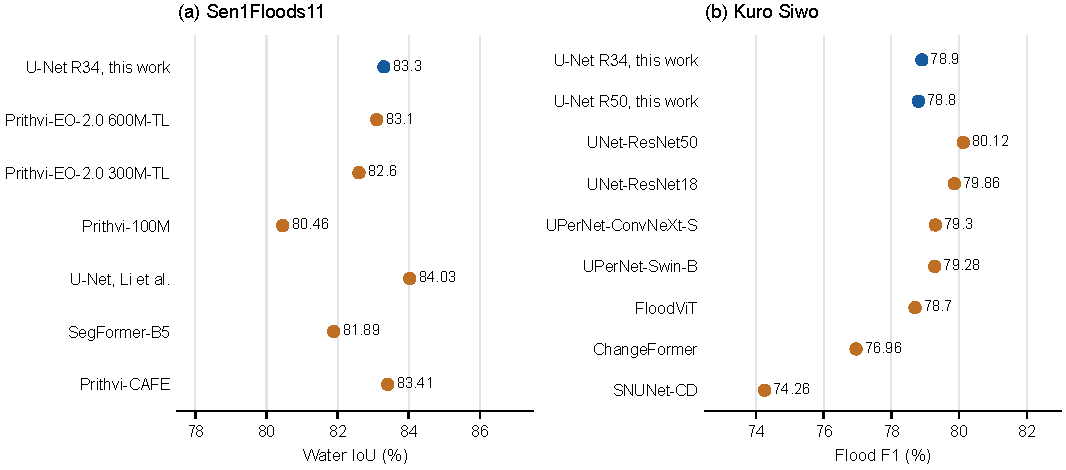
\includegraphics[width=\linewidth]{fig_model_comparison.pdf}
\caption{Water-model comparison on Sen1Floods11 (a) and Kuro Siwo (b). Blue points are this work;
orange points are published model scores. Optical values are from Szwarcman et al.~\cite{prithvi2},
the Prithvi-100M model card~\cite{prithvi1}, Li et al.~\cite{li} and Kaushik et al.~\cite{cafe}.
Radar comparisons are from Bountos et al.~\cite{kuro}. Published models were not rerun here.
The two radar models from this work were compared on the test split during model selection.}
\label{fig:model-comparison}
\end{figure*}

\subsection{Event mapping}
The combined flood map has mean F1 0.546 across 27 events, compared with 0.258 for UN-SPIDER and
0.259 for Otsu thresholding (Fig.~\ref{fig:benchmarks}; Table~\ref{tab:benchmarks}). The combined
map equals or exceeds all compared methods on 17 events. The radar--optical water union has mean F1
0.726 on the five lowland evaluation events, above the combined map's 0.704, while the mountain
evaluation gives 0.508 at K\l{}odzko and 0.262 at Cantiano. Individual event scores are shown in
Fig.~\ref{fig:event-scores}.


\begin{figure*}[!t]
\centering
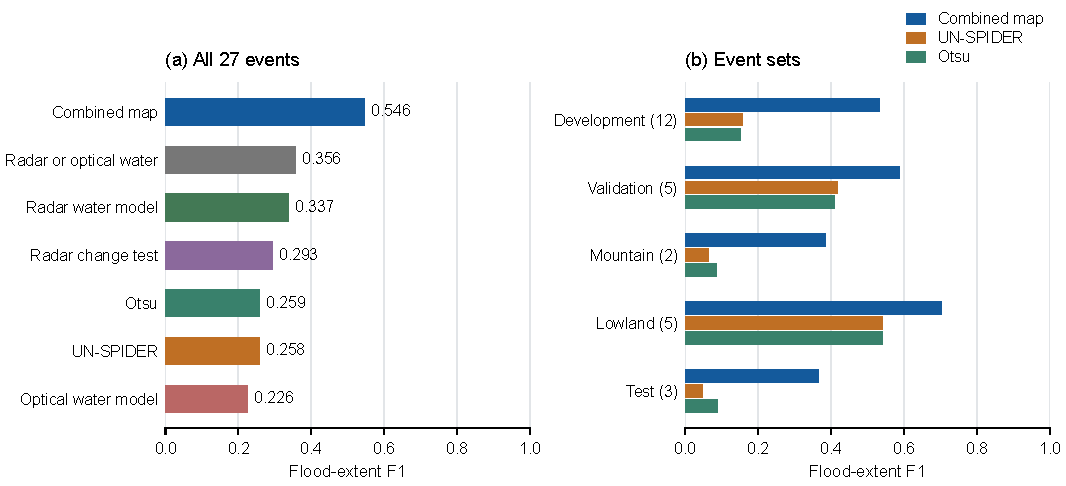
\includegraphics[width=\linewidth]{fig_benchmarks.pdf}
\caption{Mean flood-extent F1 by method (a) and event set (b). Events have equal weight.
Development, validation and lowland evaluation scores include parameter selection.}
\label{fig:benchmarks}
\end{figure*}

\begin{figure*}[!t]
\centering
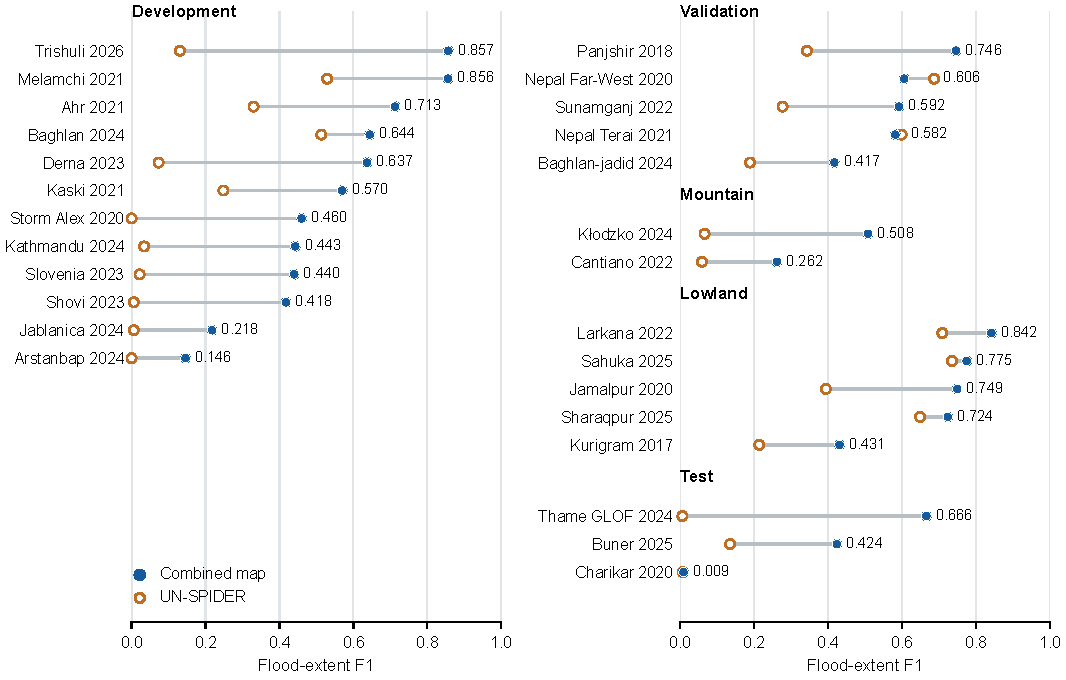
\includegraphics[width=\linewidth]{fig_event_scores.pdf}
\caption{Flood-extent F1 for the combined map and UN-SPIDER. Labels are combined-map scores.
The three test events were excluded from further parameter selection after scoring.
The snow-exclusion experiment is reported separately in Section~\ref{sec:snow}.}
\label{fig:event-scores}
\end{figure*}



The validation mean increases from 0.499 to 0.589 when the plains rule is added. On the three test
events, mean F1 is 0.366: Thame 0.666, Buner 0.424 and Charikar 0.009. With Sentinel-2 withheld, the
test mean is 0.294 (Fig.~\ref{fig:sentinel2}; Table~\ref{tab:withheld}). At Charikar, most of the
$0.25\km^2$ urban flood trace is missed, and the highest score among the tested methods is 0.04.
Narrow mudflows and hillslope landslides also give low development scores at Arstanbap (0.146) and
Jablanica (0.218).



\begin{figure*}[!t]
\centering
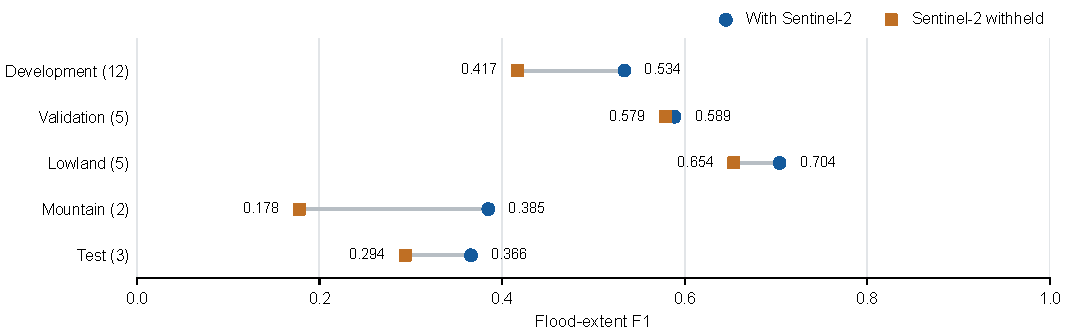
\includegraphics[width=\linewidth]{fig_sentinel2.pdf}
\caption{Mean flood-extent F1 with Sentinel-2 and with Sentinel-2 withheld. The event sets and
reference extents are unchanged between the two calculations.}
\label{fig:sentinel2}
\end{figure*}

\subsection{Optical date selection}
\label{sec:snow}
Snow-covered pixels contributed to the clear-cover fraction used to select Sentinel-2 dates,
although snow was removed when reflectance composites were made. Excluding snow raises Kaski F1 from
0.5704 to 0.5906 and decreases Melamchi from 0.8558 to 0.8546. The other ten development events keep
the same dates. Mean F1 changes from 0.5335 to 0.5351, with a paired 95\% bootstrap interval for the
change from $-0.0003$ to $+0.0051$; the interval includes zero. This comparison uses the development
events and changes only the coverage calculation, with shadow masking held fixed.

\begin{table}[!htb]
\caption{Snow exclusion in optical date selection.}
\label{tab:snow}
\fontsize{8.2}{9.6}\selectfont
\begin{tabularx}{\linewidth}{@{}Lrrr@{}}
\toprule
Area & Snow included F1 & Snow excluded F1 & F1, no S2 \\
\midrule
Twelve development events & 0.5335 & 0.5351 & 0.4168 \\
Tzermiado 2026 & 0.4772 & 0.4772 & 0.5477 \\
San Sebastiano da Po 2025 & 0.2347 & 0.2347 & 0.1020 \\
\addlinespace
Viksdalen 2024, landslide & 0.0004 & 0.0004 & 0.0000 \\
\bottomrule
\end{tabularx}
\end{table}

The snow-exclusion comparison includes two additional flood areas (Table~\ref{tab:snow}). Tzermiado uses
EMSR933 AOI03 from GeoEye-1 and San Sebastiano uses EMSR800 AOI01 from Pl\'eiades. Their selected
dates and maps are unchanged, so these flood cases show no gain from the correction. At Tzermiado,
recall is 0.905 but $10.50\km^2$ is mapped within the analysed region against $3.76\km^2$ in the
reference, giving precision 0.324. Withholding Sentinel-2 reduces the extra mapped area and
increases F1 to 0.548. The additional CPU runs omit prediction averaging over rotations and
reflections.

The Viksdalen EMSR775 AOI11 product was found to contain only one landslide polygon, with area 0.16
ha and thirteen cells on the 10 m grid. The landslide score is reported separately from the flood comparisons.

\subsection{Water segmentation and added observations}
The optical model has water IoU 0.833 and F1 0.909 on the Sen1Floods11 test split, and IoU 0.796 and
F1 0.886 on Bolivia (Table~\ref{tab:water}). Adding optical new water to the combined map increases
the twelve-event development mean F1 by 0.0066, with a paired 90\% interval from 0.0001 to 0.0138.
With Sentinel-2 withheld, estimated flood levels increase mean F1 from 0.371 to 0.417, a change of
0.046 with an interval from 0.023 to 0.073; ten events improve and none decline. Whole-map
flood-level estimates score 0.47--0.49 against 0.527 for the combined map, so the estimated level is
used only for unobserved valley ground.

\begin{table}[!htb]
\caption{Water-model test results. Kuro Siwo test scores were observed during development.}
\label{tab:water}
\fontsize{8.2}{9.6}\selectfont
\begin{tabularx}{\linewidth}{@{}Lrrrr@{}}
\toprule
Model and test set & IoU & F1 & Precision & Recall \\
\midrule
Optical U-Net, Sen1Floods11 & 0.833 & 0.909 & 0.937 & 0.883 \\
Optical U-Net, Bolivia & 0.796 & 0.886 & 0.903 & 0.870 \\
Radar ResNet-34, Kuro Siwo & \dash & 0.789 & \dash & \dash \\
Radar ResNet-50, Kuro Siwo & \dash & 0.788 & \dash & \dash \\
\bottomrule
\end{tabularx}
\end{table}

\subsection{Trishuli case study}
The Trishuli run covers $6{,}080\km^2$ and starts from raw satellite data. Its likely extent has
pooled F1 0.906 against EMSR927 AOIs 01, 02, 03 and 05, with precision 0.906 and recall 0.907
(Table~\ref{tab:trishuli}, Fig.~\ref{fig:case}). The UNOSAT corridor comparison gives F1 0.815,
precision 0.875 and recall 0.763. These are development results because Trishuli was used to select
mapping settings. On the $49.5\km^2$ where both references map the event, EMSR927 and UNOSAT agree
at F1 0.938, while the combined map scores 0.907 and 0.905 against them. UN-SPIDER scores 0.26 on
this area and the radar water model alone 0.69. At Baghlan, the Pl\'eiades and Sentinel-2 reference
maps agree at 0.845.

\begin{table}[!htb]
\caption{Trishuli comparison with EMSR927. Building and road comparisons use a 20 m tolerance.}
\label{tab:trishuli}
\fontsize{8.2}{9.6}\selectfont
\begin{tabularx}{\linewidth}{@{}Lrrrr@{}}
\toprule
Quantity & AOI01 & AOI02 & AOI03 & AOI05 \\
\midrule
Flood-extent F1 & 0.912 & 0.862 & 0.915 & 0.904 \\
Building recall & 0.68 & 0.84 & 0.81 & 0.55 \\
Building precision & 0.95 & 0.85 & 0.89 & 0.72 \\
Road-length recall & 0.76 & 0.69 & 0.88 & 0.66 \\
Road-length precision & 0.81 & 0.73 & 0.83 & 0.71 \\
\bottomrule
\end{tabularx}
\end{table}

\begin{figure*}[!t]
\centering
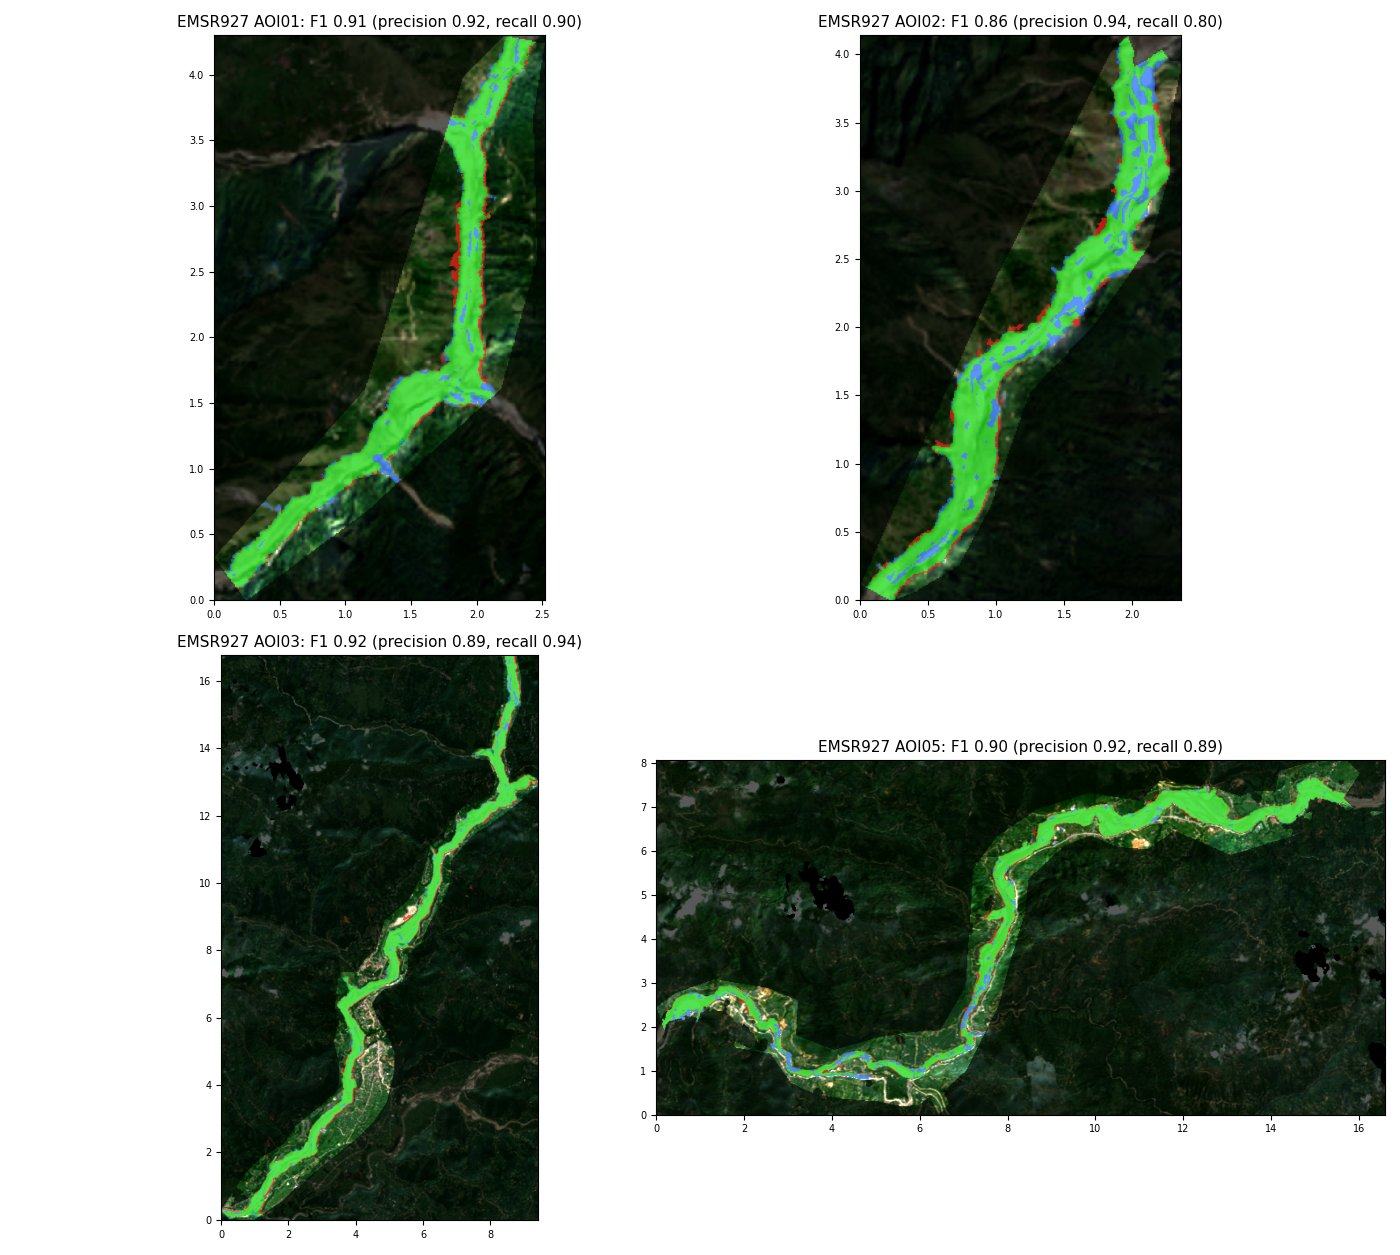
\includegraphics[width=\linewidth]{fig_case_study.jpg}
\caption{Trishuli likely extent and EMSR927 observed-event polygons. Green indicates overlap, red
the mapped extent only, and blue the EMS reference only; ground outside each analysed area is
dimmed. Background: post-event Sentinel-2 composite. Axes are in kilometres. Contains modified
Copernicus Sentinel data 2026. Reference: European Union, Copernicus Emergency Management Service
data.}
\label{fig:case}
\end{figure*}

The likely extent covers $72.1\km^2$, or $153.1\km^2$ when possible detections are included. There
are $53.4\km^2$ without observations and $4.6\km^2$ estimated beneath cloud. The likely extent
contains 3,958 buildings, with 126 km of motorable road and 60 motorable and 68 foot bridges
affected. Road access is lost for 10,788 buildings in 58 named settlements, including 4,415 without
a mapped trail avoiding the extent. Reopening 8.8 km of NH42 near Khangjim, including a bridge,
reconnects 2,993 buildings in the road calculation.

Settlement access was also calculated using EMS-graded road and bridge breaks over the same road
graph and EMS area. The buildings classified without road access agree at precision 0.874, recall
0.835 and F1 0.854 between the EMS-break and mapped-break calculations. Differences include 1,408
buildings behind breaks present only in the mapped extent and 789 behind EMS breaks classified as
possible. The mapped infrastructure damage and road access have not been checked on the ground.

\subsection{Outputs and runtime}
The dashboard contains the extent, settlements without road access, their pre-event routes and the
breaks along those routes (Fig.~\ref{fig:dashboard}). English and Nepali situation reports use the
same counts. Map data are embedded in one HTML file, while its display libraries load from the
internet. Repair candidates and settlements along a supplied upstream flow path can be inspected
with the map.

\begin{figure*}[!t]
\centering
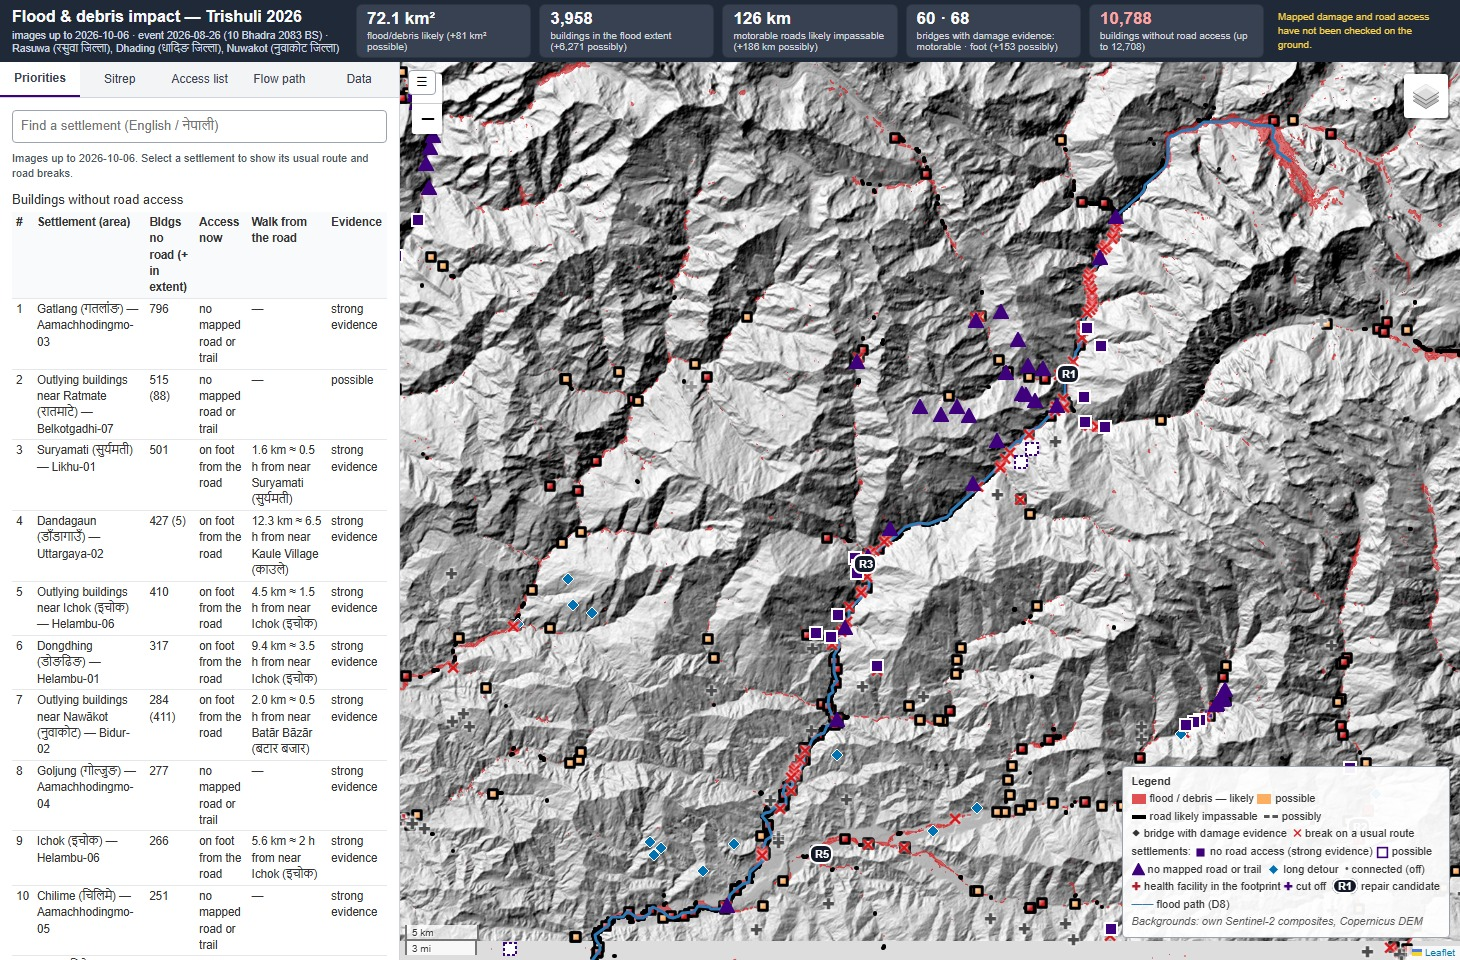
\includegraphics[width=\linewidth]{fig_dashboard.jpg}
\caption{Trishuli dashboard. The settlement list gives road access, remaining trails, walking times
and road-break evidence. Selecting a settlement displays its usual route and breaks. The map
includes likely flood extent, settlements without road access, repair candidates and the drainage
path from an upstream point. Background: Copernicus DEM hillshade.}
\label{fig:dashboard}
\end{figure*}

Raw-data runs on an eight-vCPU CPU machine take 19--46 min for areas of about 500--1,500
$\mathrm{km}^2$, and 1 h 51 min for the $6{,}080\km^2$ Trishuli box. The Sikkim GLOF of 4 October
2023 was run without selecting settings on that event and takes 36.5 min on an L4 GPU for
$1{,}311\km^2$; radar water prediction takes 3.3 min and optical water prediction 0.6 min. Its
likely extent is $13.3\km^2$, with 806 buildings without road access in Dzongu and a bridge near
Sangkalang as the first repair candidate. The Sikkim outputs have no reference-map score.

\section{Ablation studies}
Retraining radar water models with Himalayan non-flood samples reduces mean F1 by 0.103 on the
three tested Himalayan events, with an interval from $-0.155$ to $-0.050$, so those weights are not
used (Table~\ref{tab:alternatives}). Relaxed tributary connections, revised vegetation-change
detectors, supported early debris and Lee Sigma filtering before terrain correction also fail to
improve the development mean sufficiently. Excluding snow gives the small development gain in
Section~\ref{sec:snow}, while leaving the two additional flood maps unchanged.



\section{Limitations}
The Trishuli overlap was measured on a development event, while the three test events have mean F1
0.366. Validation and lowland evaluation scores include parameter selection. Most of the narrow
urban trace at Charikar was missed. Water segmentation also misses debris after water has receded,
and river restrictions can exclude small mudflows and hillslope landslides. At Kurigram, water
already present before the event produces little change and the mapped extent covers 29\% of the
reference flood area. The direct water rule improves some lowland comparisons but does not remove
these omissions.

The images used here are separated by 6--12 days, so the extent describes conditions at the
acquisition dates and cannot warn of a glacier collapse minutes ahead. Where cloud prevents an
optical observation, the extent added below the estimated river level is inferred from neighbouring
observations. Exposure of a building to this extent does not establish destruction, and building
counts do not establish population. Road access depends on pre-event OpenStreetMap coverage; Derna
has few mapped buildings, and a route remaining in the graph has not been checked on the ground.
Roads beyond the mapped area are assumed open.

Reference maps contain water, deposited debris or both, with different treatment of the river
channel and acquisition dates. Some references share a sensor or an optical acquisition with the
mapping inputs, while the five lowland evaluation references use other sensors. Areas outside the
declared analysis extent have no reference assessment. The snow correction has a small development
gain whose interval includes zero and leaves the two additional flood results unchanged; the uneven
mountain-event results remain unresolved.

\section*{Data attribution}
Contains modified Copernicus Sentinel data 2026 and 2017--2025 for the evaluation events. Produced
using Copernicus WorldDEM-30 \textcopyright{} DLR e.V. 2010--2014 and \textcopyright{} Airbus
Defence and Space GmbH 2014--2018, provided under COPERNICUS by the European Union and ESA; all
rights reserved. OpenStreetMap data: \textcopyright{} OpenStreetMap contributors, with derived
layers under ODbL. Satellite and DEM access uses Microsoft Planetary Computer, and dated
OpenStreetMap extracts use Geofabrik. Training data are Kuro Siwo and Sen1Floods11. The optical
encoder uses ImageNet-pretrained ResNet-34 through segmentation-models-pytorch. Copernicus EMS and
UNOSAT products are used for evaluation only. Claude and Codex were used to edit code and
documentation.

\begin{thebibliography}{9}
\footnotesize
\raggedright
\bibitem{kuro}
N.~I.~Bountos, M.~Sdraka, A.~Zavras et al., ``Kuro Siwo: 33 billion $\mathrm{m}^2$ under the water.
A global multi-temporal satellite dataset for rapid flood mapping,'' \textit{NeurIPS Datasets and
Benchmarks}, 2024. \url{https://arxiv.org/abs/2311.12056}.

\bibitem{sen1}
D.~Bonafilia, B.~Tellman, T.~Anderson and E.~Issenberg, ``Sen1Floods11: A georeferenced dataset to
train and test deep learning flood algorithms for Sentinel-1,'' \textit{IEEE/CVF CVPR Workshops},
2020.
\url{https://openaccess.thecvf.com/content_CVPRW_2020/html/w11/Bonafilia_Sen1Floods11_A_Georeferenced_Dataset_to_Train_and_Test_Deep_Learning_CVPRW_2020_paper.html}.

\bibitem{cems}
European Union, Copernicus Emergency Management Service, \textit{Rapid Mapping products}. EMSR927
case study; further activations used for evaluation include EMSR459, 467/468, 517, 634, 680, 696,
756, 770, 775, 800, 838 and 933. \url{https://rapidmapping.emergency.copernicus.eu/}.

\bibitem{unosat}
United Nations Satellite Centre (UNOSAT), \textit{Satellite-derived flood maps}. Products used for
evaluation include 2531, 2665, 2864, 2871, 3235, 3303, 3348, 3849 and 3919.
\url{https://unosat.org/products}.

\bibitem{unspider}
UN-SPIDER, ``Flood mapping and damage assessment using Sentinel-1 SAR data in Google Earth Engine,''
\textit{Recommended Practices}. \url{https://un-spider.org/advisory-support/recommended-practices}.

\bibitem{prithvi2}
D.~Szwarcman, S.~Roy, P.~Fraccaro et al., ``Prithvi-EO-2.0: A versatile multi-temporal foundation
model for Earth observation applications,'' arXiv:2412.02732, 2024. Table IV.
\url{https://arxiv.org/abs/2412.02732}.

\bibitem{prithvi1}
IBM--NASA Geospatial, ``Prithvi-EO-1.0-100M-sen1floods11,'' \textit{Hugging Face model card}.
\url{https://huggingface.co/ibm-nasa-geospatial/Prithvi-EO-1.0-100M-sen1floods11}.

\bibitem{li}
W.~Li, H.~Lee, S.~Wang, C.-Y.~Hsu and S.~T.~Arundel, ``Assessment of a new GeoAI foundation model
for flood inundation mapping,'' \textit{ACM SIGSPATIAL AI for Geographic Knowledge Discovery
Workshop}, 2023. Tables 2--3. \url{https://arxiv.org/abs/2309.14500}.

\bibitem{cafe}
S.~Kaushik, L.~Maurya and B.~Tellman, ``Prithvi-Complimentary Adaptive Fusion Encoder (CAFE):
unlocking full-potential for flood inundation mapping,'' arXiv:2601.02315, 2026. Table 1.
\url{https://arxiv.org/abs/2601.02315}.
\end{thebibliography}

\clearpage
\onecolumn
\appendix
\section{Evaluation tables}
\renewcommand{\arraystretch}{1.0}

\par\noindent\begin{minipage}{\linewidth}
\captionof{table}{Event sets and their use.}\label{tab:events}
\fontsize{8.2}{9.6}\selectfont
\begin{tabularx}{\linewidth}{@{}P{0.15\linewidth}P{0.46\linewidth}L@{}}
\toprule
Set & Events & Use \\
\midrule
Development (12) & Trishuli 2026, Melamchi 2021, Kaski 2021, Kathmandu 2024, Baghlan 2024, Shovi
2023, Arstanbap 2024, Storm Alex 2020, Slovenia 2023, Jablanica 2024, Ahr 2021, Derna 2023 & Change
thresholds, terrain limits, model settings and road-access rules selected on these events. \\
Validation (5) & Panjshir 2018, Baghlan-jadid 2024, Nepal Far-West 2020, Nepal Terai 2021,
Sunamganj 2022 & Three lowland events used to select the plains rule. \\
Lowland evaluation (5) & Sahuka 2025, Larkana 2022, Kurigram 2017, Sharaqpur 2025, Jamalpur 2020 &
Scores used to compare the combined radar--optical water rule. \\
Mountain evaluation (2) & K\l{}odzko 2024, Cantiano 2022 & Evaluated once per method. \\
Test (3) & Thame GLOF 2024, Buner 2025, Charikar 2020 & Excluded from parameter selection after scoring. \\
Additional floods (2) & Tzermiado 2026, San Sebastiano da Po 2025 & Snow exclusion in optical
date coverage evaluated with the remaining processing held fixed. \\
Additional landslide & Viksdalen 2024 & Landslide result reported separately from the two additional
flood cases. \\
Qualitative & Bhote Koshi 2025, Sikkim 2023 & Visual or runtime checks without a scored reference
comparison. \\
\bottomrule
\end{tabularx}
\end{minipage}\par\vspace{8pt}

\par\noindent\begin{minipage}{\linewidth}
\captionof{table}{Mean flood-extent F1 across 27 events.}
\label{tab:benchmarks}
\fontsize{8.2}{9.6}\selectfont
\begin{tabularx}{\linewidth}{@{}Lrrrrrr@{}}
\toprule
Method & \shortstack{Dev.\\(12)} & \shortstack{Validation\\(5)} & \shortstack{Mountain\\(2)} &
\shortstack{Lowland\\(5)} & \shortstack{Test\\(3)} & \shortstack{All\\(27)} \\
\midrule
Combined map & 0.534 & 0.589 & 0.385 & 0.704 & 0.366 & 0.546 \\
UN-SPIDER & 0.158 & 0.419 & 0.063 & 0.540 & 0.049 & 0.258 \\
Otsu & 0.151 & 0.409 & 0.086 & 0.542 & 0.090 & 0.259 \\
Radar change test & 0.258 & 0.445 & 0.074 & 0.383 & 0.176 & 0.293 \\
Radar water model & 0.225 & 0.535 & 0.029 & 0.667 & 0.115 & 0.337 \\
Optical water model & 0.206 & 0.166 & 0.021 & 0.515 & 0.066 & 0.226 \\
Radar or optical water & 0.238 & 0.539 & 0.029 & 0.726 & 0.126 & 0.356 \\
\bottomrule
\end{tabularx}
\end{minipage}\par\vspace{8pt}

\par\noindent\begin{minipage}{\linewidth}
\captionof{table}{Mean F1 with Sentinel-2 and with Sentinel-2 withheld.}
\label{tab:withheld}
\fontsize{8.2}{9.6}\selectfont
\begin{tabularx}{\linewidth}{@{}Lrr@{}}
\toprule
Events & With S2 & S2 withheld \\
\midrule
Development (12) & 0.534 & 0.417 \\
Validation (5) & 0.589 & 0.579 \\
Mountain evaluation (2) & 0.385 & 0.178 \\
Lowland evaluation (5) & 0.704 & 0.654 \\
Test (3) & 0.366 & 0.294 \\
\bottomrule
\end{tabularx}
\end{minipage}\par\vspace{8pt}

\par\noindent\begin{minipage}{\linewidth}
\captionof{table}{Ablation studies. Changes are paired differences in mean flood-extent F1.}
\label{tab:alternatives}
\fontsize{8.2}{9.6}\selectfont
\begin{tabularx}{\linewidth}{@{}P{0.30\linewidth}P{0.28\linewidth}L@{}}
\toprule
Method change & Evaluation & Result \\
\midrule
Himalayan non-flood samples for radar training & Three Himalayan events, HAND below 40 m &
$-0.103$ [$-0.155$, $-0.050$]. \\
Estimated flood level as the whole map & Twelve development events & F1 0.47--0.49; radar and
optical change with radar water predictions gives 0.527. \\
Add optical new water & Twelve development events & $+0.0066$ [90\% interval 0.0001, 0.0138]. \\
Estimate extent beneath cloud & Twelve development events, S2 withheld & $+0.046$ [0.023, 0.073];
ten events improve and none decline. \\
Radar water without river-connection requirement on plains & Three lowland events and fourteen
other events & Lowland changes $+0.09$ with S2 and $+0.19$ without S2; other-event mean $+0.001$. \\
Omit optical change on plains & Development events and Larkana & Development mean $+0.006$;
Larkana $-0.26$. \\
Combine radar and optical water on plains & Development lowland events; Sharaqpur and Jamalpur &
Development mean $+0.014$; two-event changes $+0.0135$ with S2 and $+0.052$ without S2. \\
River connections at 2 or $5\km^2$ & Twelve development events, four settings & Maximum mean change
$+0.0022$. \\
Calibrated or recurring vegetation change & Twelve events, four settings; prior-year imagery
available for eight & Mean changes $-0.0025$ to $+0.0009$. \\
Early debris with radar or model support & Twelve development events, two settings & Mean changes
$-0.0010$ and $-0.0017$. \\
Lee Sigma before terrain correction & Twelve development events & Mean changes $-0.0006$ with S2
and $-0.0008$ without S2. \\
Exclude snow from optical date coverage & Twelve development events and two additional flood areas &
Development mean $+0.0016$; additional flood maps unchanged. \\
\bottomrule
\end{tabularx}
\end{minipage}\par\vspace{8pt}

\par\noindent\begin{minipage}{\linewidth}
\captionof{table}{Individual-mask F1. Development and test columns are
restricted below HAND 40 m; the other columns use their reference extents. The radar change rule
differs from the calibrated radar change test in Table~\ref{tab:benchmarks}.}
\label{tab:individual}
\fontsize{8.2}{9.6}\selectfont
\begin{tabularx}{\linewidth}{@{}Lrrrr@{}}
\toprule
Mask & \shortstack{Development\\(12)} & \shortstack{Validation\\(5)} & \shortstack{Lowland\\(5)} &
\shortstack{Test\\(3)} \\
\midrule
Radar change rule & 0.323 & 0.428 & 0.427 & \dash \\
Radar water model & 0.323 & 0.535 & 0.667 & 0.190 \\
Optical water model & 0.227 & 0.166 & 0.400 & 0.076 \\
Radar or optical water & 0.350 & 0.539 & 0.716 & 0.224 \\
\bottomrule
\end{tabularx}
\end{minipage}\par\vspace{8pt}

\par\noindent\begin{minipage}{\linewidth}
\captionof{table}{Combined-map F1 by event. Snow exclusion in the date-selection coverage changes Kaski
to 0.5906 and Melamchi to 0.8546 (Section~\ref{sec:snow}).}\label{tab:event-scores}
\fontsize{8.2}{9.6}\selectfont
\begin{tabularx}{\linewidth}{@{}P{0.25\linewidth}Lr@{}}
\toprule
Set & Event & F1 \\
\midrule
Development & Trishuli 2026 & 0.857 \\
 & Melamchi 2021 & 0.856 \\
 & Ahr 2021 & 0.713 \\
 & Baghlan 2024 & 0.644 \\
 & Derna 2023 & 0.637 \\
 & Kaski 2021 & 0.570 \\
 & Storm Alex 2020 & 0.460 \\
 & Kathmandu 2024 & 0.443 \\
 & Slovenia 2023 & 0.440 \\
 & Shovi 2023 & 0.418 \\
 & Jablanica 2024 & 0.218 \\
 & Arstanbap 2024 & 0.146 \\
\addlinespace
Validation & Panjshir 2018 & 0.746 \\
 & Baghlan-jadid 2024 & 0.417 \\
 & Nepal Far-West 2020 & 0.606 \\
 & Sunamganj 2022 & 0.592 \\
 & Nepal Terai 2021 & 0.582 \\
\addlinespace
Mountain evaluation & K\l{}odzko 2024 & 0.508 \\
 & Cantiano 2022 & 0.262 \\
\addlinespace
Lowland evaluation & Sahuka 2025 & 0.775 \\
 & Larkana 2022 & 0.842 \\
 & Kurigram 2017 & 0.431 \\
 & Sharaqpur 2025 & 0.724 \\
 & Jamalpur 2020 & 0.749 \\
\addlinespace
Test & Thame GLOF 2024 & 0.666 \\*
 & Buner 2025 & 0.424 \\*
 & Charikar 2020 & 0.009 \\
\bottomrule
\end{tabularx}
\end{minipage}\par\vspace{8pt}

\par\noindent\begin{minipage}{\linewidth}
\captionof{table}{Published optical water IoU on the Sen1Floods11 hand-labelled test split, in percent.
Bolivia is absent from the training split. Values are reported by the cited sources rather than
rerun here.}
\label{tab:published-optical}
\fontsize{8.2}{9.6}\selectfont
\begin{tabularx}{\linewidth}{@{}Lrr@{}}
\toprule
Model & Test IoU (\%) & Bolivia IoU (\%) \\
\midrule
Optical U-Net, this work & 83.3 & 79.6 \\
Prithvi-EO-2.0 600M-TL~\cite{prithvi2} & 83.1 & \dash \\
Prithvi-EO-2.0 300M-TL~\cite{prithvi2} & 82.6 & \dash \\
Prithvi-100M model card~\cite{prithvi1} & 80.46 & 77.95 \\
U-Net from scratch~\cite{li} & 84.03 & 70.57 \\
SegFormer-B5~\cite{li} & 81.89 & 75.82 \\
Prithvi-CAFE~\cite{cafe} & 83.41 & 81.37 \\
\bottomrule
\end{tabularx}
\end{minipage}\par\vspace{8pt}

\par\noindent\begin{minipage}{\linewidth}
\captionof{table}{Kuro Siwo GRD flood F1, in percent. Published comparisons are from Bountos et
al.~\cite{kuro}, Table 2. The two radar members from this work were compared on this test split
during development.}
\label{tab:published-radar}
\fontsize{8.2}{9.6}\selectfont
\begin{tabularx}{\linewidth}{@{}Lr@{}}
\toprule
Model & Flood F1 (\%) \\
\midrule
ResNet-34 radar U-Net, this work & 78.9 \\
ResNet-50 radar U-Net, this work & 78.8 \\
UNet-ResNet50, best reported & 80.12 \\
UNet-ResNet18 & 79.86 \\
UPerNet-ConvNeXt-S & 79.30 \\
UPerNet-Swin-B & 79.28 \\
FloodViT & 78.70 \\
ChangeFormer & 76.96 \\
SNUNet-CD & 74.26 \\
\bottomrule
\end{tabularx}
\end{minipage}\par\vspace{8pt}
\end{document}
